\documentclass[a4paper]{report}
\title{{\LARGE The detail formulation of SCALE-LES}}
\author{Seiya Nishizawa, Hirofumi Tomita, and Team SCALE}
\date{\today}


\usepackage{graphics}
\usepackage{amsmath}

\begin{document}
\maketitle
\tableofcontents


\chapter{Introduction}
%{\bf \Large
%\begin{tabular}{ccc}
%\hline
%  Corresponding author & : & ???\\
%\hline
%\end{tabular}
%}


\section{What is SCALE}
SCALE (Scalable Computing for Advanced Library and Environment)is a basic library of weather and climate models of the earth and planets intended for widespread use.
The SCALE library was co-designed by computational science and computer science researchers.



{\bf \Large
\begin{tabular}{ccc}
\hline
  Correnspoinding author & : & Hirofumi Tomita\\
\hline
\end{tabular}
}

\section{Continuity equations}

The continuity equations for each material can be described as the flux form:
\begin{eqnarray}
&&  \frac{\partial \rho q_d}{\partial t}
+ \nabla \cdot\left(\rho q_d{\bf u}\right)  = {\rm DIFF}\left[q_d\right]
\label{eq:rho_d}\\
&&  \frac{\partial \rho q_v}{\partial t}
+ \nabla \cdot\left(\rho q_v {\bf u}\right)  = S_v + {\rm DIFF}\left[q_v\right]
\label{eq:rho_v}\\
&&  \frac{\partial \rho q_l}{\partial t}
+ \nabla \cdot\left(\rho q_l {\bf u}\right)
+ \frac{\partial \rho q_l w_l}{\partial z}=S_l + {\rm DIFF}\left[q_l\right]
\label{eq:rho_l}\\
&&  \frac{\partial \rho q_s}{\partial t}
+ \nabla \cdot\left(\rho q_s {\bf u}\right)
+ \frac{\partial \rho q_s w_s}{\partial z}=S_s + {\rm DIFF}\left[q_s\right]
\label{eq:rho_s}
\end{eqnarray}
The summation of the mass concentrations should be unit:
\begin{eqnarray}
&& q_d + q_v + q_l + q_s = 1. \label{eq:total_massconcentration}
\end{eqnarray}
The source terms of water substances should satisfy the following relation:
\begin{eqnarray}
  S_v + S_l + S_s = 0.
\end{eqnarray}
The summation of Eqs.(\ref{eq:rho_d})-(\ref{eq:rho_s}) gives the
continuity equation of total density:
\begin{eqnarray}
&&  \frac{\partial \rho}{\partial t}
+ \nabla\cdot\left(\rho{\bf u}\right)
+ \frac{\partial \rho q_l w_l}{\partial z}
+ \frac{\partial \rho q_s w_s}{\partial z}
=0, \label{eq:rhotot}
\end{eqnarray}
For this derivation,
we assume that
the operator ${ \rm DIFF}\left[\right]$ is distributive.
Using Eq.(\ref{eq:total_massconcentration}),
\begin{eqnarray}
&&  { \rm DIFF}\left[q_d\right]
+{ \rm DIFF}\left[q_v\right]
+{ \rm DIFF}\left[q_l\right]
+{ \rm DIFF}\left[q_s\right]\nonumber\\
&=&{ \rm DIFF}\left[q_d+q_v+q_l+q_s\right]
={ \rm DIFF}\left[1\right] = 0
\end{eqnarray}

\section{Momentum equations}

The momentum equations for the gas, liquid, and solid material
are described as
\begin{eqnarray}
&&  \frac{\partial \rho \left(q_d+q_v\right) {\bf u}}{\partial t}
+ \nabla \cdot \left[\rho \left(q_d+q_v\right){\bf u} \otimes {\bf u}\right]\\
&=&
-\nabla p - \left[\rho \left(q_d+q_v\right)g + (f_l+f_s)\right] {\bf e_z}\nonumber\\
&&+{\bf u} S_v +{\rm DIFF}\left[(q_d+q_v){\bf u}\right]
\label{eq:momgas}\\
&&  \frac{\partial \rho q_l {\bf u}}{\partial t}
+ \nabla \cdot \left(\rho q_l{\bf u} \otimes {\bf u}\right)
+ \frac{\partial \rho q_l {\bf u} w_l}{\partial z}
=
 - \left(\rho q_l g - f_l\right) {\bf e_z}\nonumber\\
&&+{\bf u} S_l+{\rm DIFF}\left[q_l{\bf u}\right]
\label{eq:momliquid}\\
&&  \frac{\partial \rho q_s {\bf u}}{\partial t}
+ \nabla \cdot \left(\rho q_s{\bf u} \otimes {\bf u}\right)
+ \frac{\partial \rho q_s {\bf u }w_s}{\partial z}
=
 - \left(\rho q_s g - f_s\right) {\bf e_z}\nonumber\\
&&+{\bf u} S_s+{\rm DIFF}\left[q_s{\bf u}\right]
\label{eq:momsolid}
\end{eqnarray}
The pressure is derived from the equation of state as
\begin{eqnarray}
p=\rho \left(q_d R_d + q_v R_v\right) T.\label{eq:state}
\end{eqnarray}
The summation of Eqs.(\ref{eq:momgas})-(\ref{eq:momsolid})
gives the total momentum equation as
\begin{eqnarray}
&&  \frac{\partial \rho {\bf u}}{\partial t}
+ \nabla \cdot \left(\rho{\bf u} \otimes {\bf u}\right)
+ \left(\frac{\partial \rho q_l w_l}{\partial z}
+ \frac{\partial \rho q_s w_s}{\partial z}\right) {\bf e_z}\nonumber\\
&=&
-\nabla p - \rho g {\bf e_z}
+{\rm DIFF}\left[{\bf u}\right]
\label{eq:momtot}
\end{eqnarray}
Note that the drag forces by water loading does not appear
in Eq.(\ref{eq:momtot}),
because those term are cancelled out through the summation.

\section{Thermodynamics equations}

The equations of the internal energies are described as
\begin{eqnarray}
&&  \frac{\partial \rho (q_d e_d + q_v e_v) }{\partial t} +
  \nabla \cdot \left[ \rho (q_d e_d + q_v e_v ){\bf u} \right] \nonumber\\
&=& - p \nabla \cdot {\bf u} + Q_{d}+ Q_{v} + {\rm DIFF}\left[(q_d+q_v)T^{*} \right]
\label{eq:thermogas}\\
&&  \frac{\partial \rho q_l e_l}{\partial t} +
  \nabla \cdot \left( \rho q_l e_l {\bf u} \right)
+ \frac{\partial \rho q_l e_l w_l}{\partial z}
= Q_l + {\rm DIFF}\left[q_l T^{*} \right]
\label{eq:thermoliquid}\\
&&  \frac{\partial \rho q_l e_s}{\partial t} +
  \nabla \cdot \left( \rho q_s e_s {\bf u} \right)
+ \frac{\partial \rho q_s e_s w_s}{\partial z}
= Q_s + {\rm DIFF}\left[q_s T^{*} \right]
\label{eq:thermosolid}
\end{eqnarray}
where $T^*$ is some kind of potential temperature, discussed later.
The internal energies are defined as
\begin{eqnarray}
&& e_d = c_{vd} T\\
&& e_v = c_{vv} T\\
&& e_l = c_{l} T\\
&& e_s = c_{s} T,
\end{eqnarray}
The summation of Eqs.(\ref{eq:thermogas})-(\ref{eq:thermosolid})
gives the following internal energy equations:
\begin{eqnarray}
&&  \frac{\partial \rho e  }{\partial t}
+  \nabla \cdot \left( \rho e {\bf u} \right)
+ \frac{\partial \rho q_l e_l w_l}{\partial z}
 + \frac{\partial \rho q_s e_s w_s}{\partial z}
 + p \nabla \cdot {\bf u}\nonumber\\
&=&  Q + {\rm DIFF}\left[T^{*} \right]
\label{eq:etot}
\end{eqnarray}
where
\begin{eqnarray}
&&  e = q_d e_d + q_v e_v + q_l e_l + q_s e_s,
\end{eqnarray}
and the total diabatic heating is described as
\begin{eqnarray}
&&  Q = Q_d + Q_v + Q_l + Q_s.
\end{eqnarray}

\section{Conseptual seperation for solving the set of equations}

Eqs.(\ref{eq:rho_v})-(\ref{eq:rho_s}),(\ref{eq:rhotot}),(\ref{eq:momtot}),
and (\ref{eq:state}) with Eq.(\ref{eq:etot}) are the complete set of equations.
For solving them easily, we seperate the set of equations conceptually as
\begin{eqnarray}
&&  \frac{\partial \phi}{\partial t} =
\left(\frac{\partial \phi}{\partial t}\right)_{dynamics}
+\left(\frac{\partial \phi}{\partial t}\right)_{physics}
\end{eqnarray}
The falling proccess of liquid and solid waters,
the source and sink process of water vapor, and
the diabatic heating process for energy equations are treated
as physical process, the others are treated as dynamical proccess.

According to this scheme,
the dynamical process can be written as
\begin{eqnarray}
&&  \frac{\partial \rho q_v}{\partial t}
+ \nabla \cdot\left(\rho q_v {\bf u}\right)  = 0
\label{eq:rho_v_d}\\
&&  \frac{\partial \rho q_l}{\partial t}
+ \nabla \cdot\left(\rho q_l {\bf u}\right) = 0
\label{eq:rho_l_d}\\
&&  \frac{\partial \rho q_s}{\partial t}
+ \nabla \cdot\left(\rho q_s {\bf u}\right)
= 0
\label{eq:rho_s_d}\\
&&  \frac{\partial \rho}{\partial t}
+ \nabla\cdot\left(\rho{\bf u}\right)
=0 \label{eq:rhotot_d}\\
&&  \frac{\partial \rho {\bf u}}{\partial t}
+ \nabla \cdot \left(\rho{\bf u} \otimes {\bf u}\right)
=
-\nabla p - \rho g {\bf e_z} \label{eq:momtot_d}\\
&&  \frac{\partial \rho e  }{\partial t}
+  \nabla \cdot \left( \rho e {\bf u} \right)
 + p \nabla \cdot {\bf u}
=  0 \label{eq:etot_d}
\end{eqnarray}

On the other hand,
the physical processes are as follows:
\begin{eqnarray}
&&  \frac{\partial \rho q_v}{\partial t}  = S_v
+{\rm DIFF}\left[q_v \right]
\label{eq:rho_v_p}\\
&&  \frac{\partial \rho q_l}{\partial t}
+ \frac{\partial \rho q_l w_l}{\partial z}=S_l
+{\rm DIFF}\left[q_l \right]
\label{eq:rho_l_p}\\
&&  \frac{\partial \rho q_s}{\partial t}
+ \frac{\partial \rho q_s w_s}{\partial z}=S_s
+{\rm DIFF}\left[q_s \right]
\label{eq:rho_s_p}\\
&&  \frac{\partial \rho}{\partial t}
+ \frac{\partial \rho q_l w_l}{\partial z}
+ \frac{\partial \rho q_s w_s}{\partial z}
=0 \label{eq:rhotot_p}\\
&&  \frac{\partial \rho {\bf u}}{\partial t}
+ \frac{\partial \rho q_l {\bf u} w_l}{\partial z}
+ \frac{\partial \rho q_s {\bf u} w_s}{\partial z}
= {\rm DIFF}\left[{\bf u} \right]
 \label{eq:momtot_p}\\
&&  \frac{\partial \rho e  }{\partial t}
+ \frac{\partial \rho q_l e_l w_l}{\partial z}
 + \frac{\partial \rho q_s e_s w_s}{\partial z}
=  Q + {\rm DIFF}\left[T^{*} \right] \label{eq:etot_p}
\end{eqnarray}

\section{Conservation of thermodynamics in the dynamical process}

Equation (\ref{eq:etot_d}) is not a complete flux form,
because the internal energy itself is not conserved
both in the Euler sense and in the Lagrangian sense.
In this section, we consider the conservative
quantity for thermodynamics equation.

In the dry atmosphere, the potential temperature for dry air,
which is defined as
\begin{eqnarray}
\theta_d &=& T \left(\frac{p_{00}}{p}\right)^{R_d/c_{pd}},
\end{eqnarray}
is used as a conserved quantity it is conserved along the Lagrange trajectory
$c_{pd}$ $R_d$ are the specific heats at constant pressure and
However, it is no longer satisfied when the water substances are included.

Sinece Eq.(\ref{eq:rhotot_d}) is equivallent to
\begin{eqnarray}
  \frac{d \rho}{dt}+\rho \nabla \cdot {\bf u} = 0,
\end{eqnarray}
Equation (\ref{eq:etot_d}) is
\begin{eqnarray}
  \rho \frac{de}{dt} - \frac{p}{\rho}\frac{d \rho}{dt} =0. \label{eq:etot_d2}
\end{eqnarray}
Dividing by $\rho$, this equation can be written as
\begin{eqnarray}
  \frac{de}{dt} + p \frac{d}{dt}\left(\frac{1}{\rho}\right) = 0.
\label{eq:thermodyn}
\end{eqnarray}
Substiting Eq.(\ref{eq:state}) into Eq.(\ref{eq:thermodyn}),
\begin{eqnarray}
&& \frac{d  q_d c_{vd}   T}{dt} + p \frac{d}{dt} \left[\frac{q_d R_d T}{p}\right]
+\frac{d  q_v c_{vv}   T}{dt} + p \frac{d}{dt} \left[\frac{q_v R_v T}{p}\right]
\nonumber\\
&&+\frac{d  q_l c_{l}   T}{dt}+\frac{d  q_s c_{s}   T}{dt} =0
\label{eq:thermodyn_dash}
\end{eqnarray}

Since Eqs.(\ref{eq:rho_v_d})-(\ref{eq:rhotot_d}) give
\begin{eqnarray}
  \frac{d q_d}{dt} = \frac{d q_v}{dt} = \frac{d q_l}{dt} = \frac{d q_s}{dt} = 0,
\end{eqnarray}
Equation (\ref{eq:thermodyn_dash}) gives the following form:
\begin{eqnarray}
&& q_d  \left[\frac{d  c_{vd}   T}{dt} +  p \frac{d}{dt} \left[\frac{ R_d T}{p}\right]\right]
+q_v \left[\frac{d  c_{vv}   T}{dt} + p \frac{d}{dt} \left[\frac{ R_v T}{p}\right]\right]\nonumber\\
&&+ q_l  \frac{d  c_{l}   T}{dt} + q_s  \frac{d  c_{s}   T}{dt} =0
\end{eqnarray}
Dividing this equation by $T$,
\begin{eqnarray}
%1
&&q_d  \left[c_{pd} \frac{1}{T}\frac{d T}{dt}
+  R_d p \frac{d}{dt} \left(\frac{1}{p}\right)\right]
+q_v  \left[c_{pv} \frac{1}{T}\frac{d T}{dt}
+  R_v p \frac{d}{dt} \left(\frac{1}{p}\right)\right]\nonumber\\
&&+ q_l c_{l} \frac{1}{T}  \frac{d   T}{dt}
  + q_s c_{s} \frac{1}{T}  \frac{d   T}{dt} =0\\
%2
&&q_d c_{pd} \left[ \frac{d \ln T}{dt}
+  \frac{R_d}{c_{pd}} \frac{d}{dt} \left[\ln \left(\frac{1}{p}\right)\right]\right]
+q_v c_{pv}  \left[\frac{d \ln T}{dt}
+  \frac{R_v}{c_{pv}} \frac{d}{dt} \left[\ln \left(\frac{1}{p}\right)\right]\right]\nonumber\\
&&+ q_l c_{l}  \frac{d \ln T}{dt}
  + q_s c_{s}  \frac{d \ln T}{dt} =0 \label{eq:thermdyn2}\\
&&
 q_d c_{pd} \frac{d \ln \theta_d}{dt}
+q_v c_{pv} \frac{d \ln \theta_v}{dt}
+q_l c_l   \frac{d \ln T}{dt}
+q_s c_s   \frac{d  \ln T}{dt}=0\\
&&
\frac{d}{dt}\left[ \ln \left(
\theta_d^{q_d c_{pd}} \theta_v^{q_v c_{pv}} T^{q_l c_l} T^{q_s c_s}
\right)\right] = 0 \label{eq:lnThetaconserveation}
\end{eqnarray}
Thus,
\begin{eqnarray}
&&\frac{d}{dt}\left[
\theta_d^{q_d c_{pd}} \theta_v^{q_v c_{pv}} T^{q_l c_l} T^{q_s c_s}
\right] = 0
\end{eqnarray}
Thus, the following quantity is conserved along the flow trajectory;
\begin{eqnarray}
\Theta = \theta_d^{q_d c_{pd}} \theta_v^{q_v c_{pv}} T^{q_l c_l} T^{q_s c_s}
\end{eqnarray}
where $\theta_v$ is the potential temperature for water vapor, defined as
\begin{eqnarray}
\theta_v &=& T \left(\frac{p_{00}}{p}\right)^{R_v/c_{pv}}
\end{eqnarray}

The equation of state has the following expression using $\Theta$.
\begin{eqnarray}
\Theta &=&
T^{q_d c_{pd}} \left(\frac{p_{00}}{p}\right)^{q_d R_d}
T^{q_v c_{pv}} \left(\frac{p_{00}}{p}\right)^{q_v R_v}
T^{q_l c_l}  + T^{q_s c_s} \\
&=&
T^{q_d c_{pd} +q_vc_{pv}+q_lc_l+q_sc_s}
\left(\frac{p_{00}}{p}\right)^{q_d R_d + q_v R_v} \\
&=&
T^{c_p^*}\left(\frac{p_{00}}{p}\right)^{R^*},
\end{eqnarray}
where
\begin{eqnarray}
  c_p^* &\equiv& q_d c_{pd} +q_vc_{pv}+q_lc_l+q_sc_s\\
  R^* &\equiv& q_d R_d + q_v R_v
\end{eqnarray}
We define a new potential temperature
\begin{eqnarray}
\theta \equiv \Theta^{1/c_p^*} &=& T \left(\frac{p_{00}}{p}\right)^{R^*/c_p^*}
%&=& T \left(\frac{p_{00}}{p}\right)^{\frac{R_d}{c_{pd}} \alpha}
\end{eqnarray}
%% where
%% \begin{eqnarray}
%%   \alpha &=& \frac{q_d + q_v \frac{R_v}{R_d}}{q_d + q_v \frac{c_{pv}}{c_{pd}}+q_l\frac{c_l}{c_{pd}}
%% +q_s\frac{c_s}{c_{pd}}}
%% \end{eqnarray}

The pressure expression is derived diagnostically as follows:
\begin{eqnarray}
p&=&\rho (q_d R_d + q_v R_v) \theta \left(\frac{p}{p_{00}}\right)^{\frac{R^*}{c_{p}^*}}\\
p^{1-\frac{R^*}{c_{p}^*}}&=&\rho R^* \theta \left(\frac{1}{p_{00}}\right)^{\frac{R^*}{c_{p}^*}}\\
p&=&p_{00}\left(\frac{\rho \theta R^*}{p_{00}} \right)^{\frac{c_{p}^*}{c_{p}^*- R^*}} \label{eq: pressure}
\end{eqnarray}

Note that
\begin{eqnarray}
  \frac{d \theta}{dt} = \frac{1}{a} \Theta^{1/a-1} \frac{d \Theta}{dt} = 0
  \label{eq:theta_theta_relation}
\end{eqnarray}
Therefore, $\rho \theta$ can be employed for the prognostic varaiable!

Figure \ref{fig:fig1}(a) gives the vertical profile of the temperature
in the U.S.standard atmosphere and Fig.\ref{fig:fig1}(b) shows
the vetical profiles of $\theta/\theta_d$ under this temperature condition
when we assume that $q_v$ is mass concentration of water vapor at the saturation,
$q_l+q_s$ gives 0.0, 0.01, 0.02, and 0.04.
The differnce between $\theta$ and $\theta_d$ becomes
larger with the height and it may not be negligible.

\section{Diabatic heating in the physical process}

If the prognostic variable for thermodynamics is changed
from the internal energy to the newly defined potential temperature $\theta$,
the diabatic heating in Eq.(\ref{eq:etot_p}) should be modified.
Through
the manupulation from Eq.(\ref{eq:etot_d2}) to Eq.(\ref{eq:lnThetaconserveation}),
Eq.(\ref{eq:etot_p}) without turbulence term can be written as
\begin{eqnarray}
  \frac{d \ln \Theta}{dt} = \frac{Q}{\rho T}
  \label{eq:dlntheta_dt}
\end{eqnarray}
On the other hand, Eq.(\ref{eq:theta_theta_relation}) gives
\begin{eqnarray}
  \frac{d \theta}{dt} = \frac{1}{c_p^*} \Theta^{1/a} \frac{d \ln \Theta}{dt}
  \label{eq:dtheta_dt}
\end{eqnarray}
Substituting Eq.(\ref{eq:dlntheta_dt}) into Eq.(\ref{eq:dtheta_dt}),
\begin{eqnarray}
  \frac{d \theta}{dt} = \frac{1}{c_p^*}
  \left(\frac{p_{00}}{p}\right)^{\frac{R^*}{c_p^*}} \frac{Q}{\rho}
\end{eqnarray}

\section{Summary of equations in the dynamical process and physical process}
\subsection{The dynamical process}
\begin{eqnarray}
&&  \frac{\partial \rho q_v}{\partial t}
+ \nabla \cdot\left(\rho q_v {\bf u}\right) = \left(\frac{\partial \rho q_v}{\partial t}\right)_{physics}
\label{eq:rho_v_d2}\\
&&  \frac{\partial \rho q_l}{\partial t}
+ \nabla \cdot\left(\rho q_l {\bf u}\right) = \left(\frac{\partial \rho q_l}{\partial t}\right)_{physics}
\label{eq:rho_l_d2}\\
&&  \frac{\partial \rho q_s}{\partial t}
+ \nabla \cdot\left(\rho q_s {\bf u}\right)
= \left(\frac{\partial \rho q_s}{\partial t}\right)_{physics}
\label{eq:rho_s_d2}\\
&&  \frac{\partial \rho}{\partial t}
+ \nabla\cdot\left(\rho{\bf u}\right)
= \left(\frac{\partial \rho}{\partial t}\right)_{physics}
 \label{eq:rhotot_d2}\\
&&  \frac{\partial \rho {\bf u}}{\partial t}
+ \nabla \cdot \left(\rho{\bf u} \otimes {\bf u}\right)
=
-\nabla p - \rho g {\bf e_z}
+\left(\frac{\partial \rho {\bf u}}{\partial t}\right)_{physics}
 \label{eq:momtot_d2}\\
&&  \frac{\partial \rho \theta  }{\partial t}
+  \nabla \cdot \left( \rho \theta {\bf u} \right) =
\left(\frac{\partial \rho \theta}{\partial t}\right)_{physics} \\
&& p=p_{00}\left(\frac{\rho \theta R^*}{p_{00}} \right)^{\frac{c_{p}^*}{c_{p}^*- R^*}}
\end{eqnarray}
where
\begin{eqnarray}
  c_p^* &\equiv& q_d c_{pd} +q_vc_{pv}+q_lc_l+q_sc_s\\
  R^* &\equiv& q_d R_d + q_v R_v
\end{eqnarray}

\subsection{The physical process}
\begin{eqnarray}
&& \left( \frac{\partial \rho q_v}{\partial t} \right)_{physics}  = S_v
+{\rm DIFF}\left[q_v \right]
\label{eq:rho_v_p2}\\
&& \left( \frac{\partial \rho q_l}{\partial t} \right)_{physics}
= - \frac{\partial \rho q_l w_l}{\partial z}+S_l
+{\rm DIFF}\left[q_l \right]
\label{eq:rho_l_p2}\\
&& \left( \frac{\partial \rho q_s}{\partial t} \right)_{physics}
=- \frac{\partial \rho q_s w_s}{\partial z}+S_s
+{\rm DIFF}\left[q_s \right]
\label{eq:rho_s_p2}\\
&& \left( \frac{\partial \rho}{\partial t} \right)_{physics}
=- \frac{\partial \rho q_l w_l}{\partial z}
 - \frac{\partial \rho q_s w_s}{\partial z}
 \label{eq:rhotot_p2}\\
&& \left( \frac{\partial \rho {\bf u}}{\partial t} \right)_{physics}
=
- \frac{\partial \rho q_l {\bf u} w_l}{\partial z}
- \frac{\partial \rho q_s {\bf u} w_s}{\partial z}
+{\rm DIFF}\left[{\bf u} \right]
 \label{eq:momtot_p2}\\
&& \left( \frac{\partial \rho \theta  }{\partial t} \right)_{physics}
=  \frac{1}{c_p^*} \left(\frac{p_{00}}{p}\right)^{\frac{R^*}{c_p^*}}
\left[Q
 - \frac{\partial \rho q_l e_l w_l}{\partial z}
 - \frac{\partial \rho q_s e_s w_s}{\partial z}
\right]
 + {\rm DIFF}\left[\theta \right] \label{eq:etot_p2}
\end{eqnarray}

\begin{figure}[t]
  (a)\\
  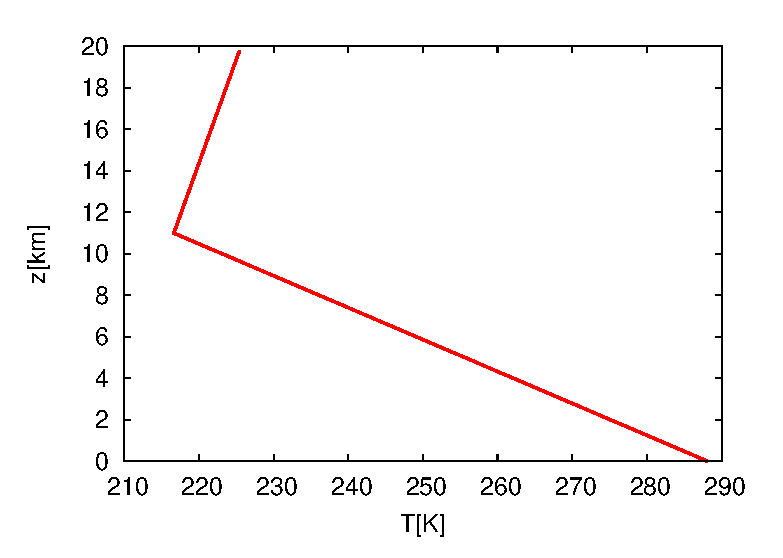
\includegraphics{./figure/us_std_atm_profile.eps}\\
  (b)\\
  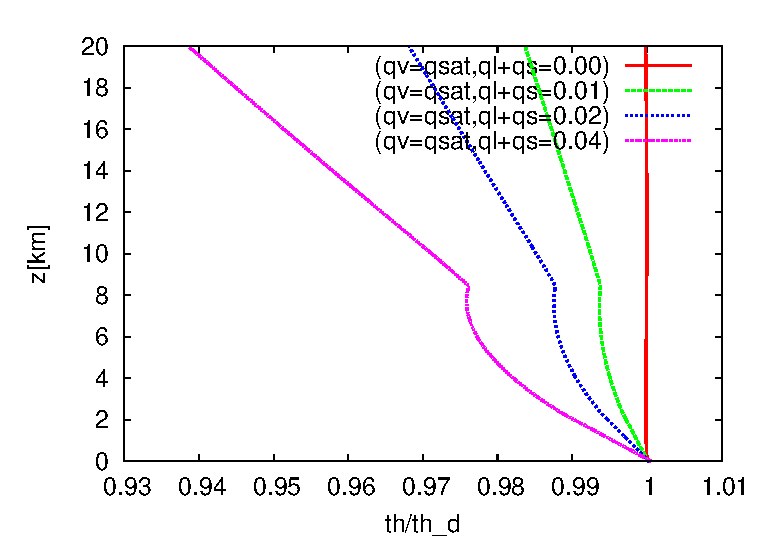
\includegraphics{./figure/theta_theta_d_profile.eps}\\
  \caption{Thee vertical profile of (a) U.S. standard atmosphere,
  (b) Several profiles of $\theta/\theta_d$.}
  \label{fig:fig1}
\end{figure}


\chapter{Descretization of the dynamics}
{\bf \Large 
\begin{tabular}{ccc}
\hline
  Corresponding author & : & Hirofumi Tomita\\
\hline
\end{tabular}
}

\section{Time integration method}

For the time integration of Eqs.(\ref{eq:rhotot_d2})-(\ref{eq:etot_d2}),
we adopt the full explicit scheme with
the $p$-th order Runge-Kutta scheme.
\begin{eqnarray}
&&  \phi^{*} = \phi^{t} - \left(\frac{\partial \phi}{\partial t}\right)^{t}\frac{\Delta t}{p}\\
&&  \phi^{**} = \phi^{t} - \left(\frac{\partial \phi}{\partial t}\right)^{*}\frac{\Delta t}{p-1}\\
&&  \cdot \cdot \cdot\nonumber\\
&&  \cdot \cdot \cdot\nonumber\\
&&  \cdot \cdot \cdot\nonumber\\
&&  \phi^{t+\Delta t} = \phi^{t} - \left(\frac{\partial \phi}{\partial t}\right)^{**\cdot\cdot\cdot\cdot*} \Delta t
\end{eqnarray}
Usually, we use $p=2,3$ and $4$.

%% HEVE full explicit
%% HEVI 
%% HIVI full implicit

\section{Spatial descretization}
We employ the Arakawa-C staggered grid with the 3-dimensional momentum 
($\rho u, \rho v, \rho w$), density ($\rho$) and mass-weighted potentail temperature($\rho \theta$)
as the prognostic variables.
Figure \ref{fig:cntrl-volume}(a) shows the structure of the control volume for the mass,
indicating the location of each of prognostic variables.
Conceptually, we use the 4th order central difference scheme 
for the advection or convection terms and
the 2nd order central difference scheme for the other terms.
Before the descretization of differential equations,
we should diagnose several quantities from the prognostic variables.
\begin{description}
\item[Full-level pressure and potential temperature]
\begin{eqnarray}
&&p_{i,j,k}=p_{00}\left[\frac{(\rho \theta)_{i,j,k} R^*}{p_{00}} \right]^{\frac{c_{p}^*}{c_{p}^*- R^*}}\\
&&\theta_{i,j,k} = \frac{(\rho \theta)_{i,j,k}}{\rho_{i,j,k}}\\
\end{eqnarray}
\item[Half-level density]
\begin{eqnarray}
&&  \overline{\rho}_{i+\frac{1}{2},j,k} = \frac{\rho_{i+1,j,k}+\rho_{i,j,k}}{2}\\
&&  \overline{\rho}_{i,j+\frac{1}{2},k} = \frac{\rho_{i,j+1,k}+\rho_{i,j,k}}{2}\\
&&  \overline{\rho}_{i,j,k+\frac{1}{2}} = \frac{\rho_{i,j,k+1}+\rho_{i,j,k}}{2}\\
\end{eqnarray}
\item[Half-level velocity]
\begin{eqnarray}
&&  \overline{u}_{i+\frac{1}{2},j,k} = \frac{(\rho u)_{i+\frac{1}{2},j,k}}{\overline{\rho}_{i+\frac{1}{2},j,k}}\\
&&  \overline{v}_{i,j+\frac{1}{2},k} = \frac{(\rho v)_{i,j+\frac{1}{2},k}}{\overline{\rho}_{i,j+\frac{1}{2},k}}\\
&&  \overline{w}_{i,j,k+\frac{1}{2}} = \frac{(\rho w)_{i,j,k+\frac{1}{2}}}{\overline{\rho}_{i,j,k+\frac{1}{2}}}
\end{eqnarray}
\item[Full-level velocity]
\begin{eqnarray}
&&  \overline{u}_{i,j,k} = \frac{(\rho u)_{i+\frac{1}{2},j,k}+(\rho u)_{i-\frac{1}{2},j,k}}{2\rho_{i,j,k}}\\
&&  \overline{v}_{i,j,k} = \frac{(\rho v)_{i,j+\frac{1}{2},k}+(\rho v)_{i,j-\frac{1}{2},k}}{2\rho_{i,j,k}}\\
&&  \overline{w}_{i,j,k} = \frac{(\rho w)_{i,j,k+\frac{1}{2}}+(\rho w)_{i,j,k-\frac{1}{2}}}{2\rho_{i,j,k}}
\end{eqnarray}
\end{description}




\subsection{Continuity equation}
\begin{eqnarray}
%%
\left(\frac{\partial \rho}{\partial t}\right)_{i,j,k}
&=& - \frac{(\rho u)_{i+\frac{1}{2},j,k} -(\rho u)_{i-\frac{1}{2},j,k}}{\Delta x}\nonumber\\
& & - \frac{(\rho v)_{i,j+\frac{1}{2},k} -(\rho v)_{i,j-\frac{1}{2},k}}{\Delta y}\nonumber\\
& & - \frac{(\rho w)_{i,j,k+\frac{1}{2}} -(\rho w)_{i,j,k-\frac{1}{2}}}{\Delta z}
\end{eqnarray}

\subsection{Momentum equations}
Figure \ref{fig:cntrl-volume}(a) shows the structure of the control volume for the momentum
in the x direction.
The momentum equation is descretized as
\begin{eqnarray}
%%
\left(\frac{\partial \rho u}{\partial t}\right)_{i+\frac{1}{2},j,k}
&=& - \frac{\overline{(\rho u)}_{i+1,j,k} \overline{u}_{i+1,j,k} 
           -\overline{(\rho u)}_{i,j,k} \overline{u}_{i,j,k}}
     {\Delta x}\nonumber\\
& & - \frac{\overline{(\rho u)}_{i+\frac{1}{2},j+\frac{1}{2},k}  \overline{v}_{i+\frac{1}{2},j+\frac{1}{2},k} 
           -\overline{(\rho u)}_{i+\frac{1}{2},j-\frac{1}{2},k}  \overline{v}_{i+\frac{1}{2},j-\frac{1}{2},k}}
     {\Delta y}\nonumber\\
& & - \frac{\overline{(\rho u)}_{i+\frac{1}{2},j,k+\frac{1}{2}}  \overline{v}_{i+\frac{1}{2},j,k+\frac{1}{2}} 
           -\overline{(\rho u)}_{i+\frac{1}{2},j,k-\frac{1}{2}}  \overline{v}_{i+\frac{1}{2},j,k-\frac{1}{2}}}
     {\Delta z}\nonumber\\
& & -\frac{p_{i+1,j,k}-p_{i,j,k}}{\Delta x},
\end{eqnarray}
where 
\begin{eqnarray}
&& \overline{(\rho u)}_{i,j,k} \nonumber\\
= && \frac{-(\rho u)_{i+\frac{3}{2},j,k}+7(\rho u)_{i+\frac{1}{2},j,k}+7(\rho u)_{i-\frac{1}{2},j,k}-(\rho u)_{i-\frac{3}{2},j,k}}{12}\\
&& \overline{(\rho u)}_{i+\frac{1}{2},j+\frac{1}{2},k} \nonumber\\
= && \frac{-(\rho u)_{i+\frac{1}{2},j+2,k}+7(\rho u)_{i+\frac{1}{2},j+1,k}+7(\rho u)_{i+\frac{1}{2},j,k}-(\rho u)_{i+\frac{1}{2},j-1,k}}{12}\\
&& \overline{(\rho u)}_{i+\frac{1}{2},j,k+\frac{1}{2}} \nonumber\\
= &&\frac{-(\rho u)_{i+\frac{1}{2},j,k+2}+7(\rho u)_{i+\frac{1}{2},j,k+1}+7(\rho u)_{i+\frac{1}{2},j,k}-(\rho u)_{i+\frac{1}{2},j,k-1}}{12}
\end{eqnarray}
and the velocities at the cell wall for the staggered control volume to $x$ direction are
defined as
\begin{eqnarray}
\overline{u}_{i,j,k} &=& \frac{\overline{u}_{i+\frac{1}{2},j,k}+\overline{u}_{i-\frac{1}{2},j,k}}{2}\\
\overline{v}_{i+\frac{1}{2},j+\frac{1}{2},k} &=& 
\frac{\overline{v}_{i,j+\frac{1}{2},k}+\overline{v}_{i+1,j+\frac{1}{2},k}}{2}\\
\overline{w}_{i+\frac{1}{2},j,k+\frac{1}{2}} &=& 
\frac{\overline{w}_{i,j,k+\frac{1}{2}}+\overline{w}_{i+1,j,k+\frac{1}{2}}}{2}
\end{eqnarray}
In this form, the 4th order accuracy is guaranteed 
on the condition of the constant velocity.

The momentum equations in the $y$ and $z$ directions are descretized 
in the same way:
\begin{eqnarray}
%%
\left(\frac{\partial \rho v}{\partial t}\right)_{i,j+\frac{1}{2},k}
&=& - \frac{\overline{(\rho v)}_{i+\frac{1}{2},j+\frac{1}{2},k}  \overline{u}_{i+\frac{1}{2},j+\frac{1}{2},k} 
           -\overline{(\rho v)}_{i-\frac{1}{2},j+\frac{1}{2},k}  \overline{u}_{i-\frac{1}{2},j+\frac{1}{2},k}}
     {\Delta x}\nonumber\\
& & - \frac{\overline{(\rho v)}_{i,j+1,k} \overline{v}_{i,j+1,k} 
           -\overline{(\rho v)}_{i,j,k} \overline{v}_{i,j,k}}
     {\Delta y}\nonumber\\
& & - \frac{\overline{(\rho v)}_{i,j+\frac{1}{2},k+\frac{1}{2}}  \overline{v}_{i,j+\frac{1}{2},k+\frac{1}{2}} 
           -\overline{(\rho v)}_{i,j+\frac{1}{2},k-\frac{1}{2}}  \overline{v}_{i,j+\frac{1}{2},k-\frac{1}{2}}}
     {\Delta z}\nonumber\\
& & -\frac{p_{i,j+1,k}-p_{i,j,k}}{\Delta y},\\
%%
\left(\frac{\partial \rho w}{\partial t}\right)_{i,j,k+\frac{1}{2}}
&=& - \frac{\overline{(\rho w)}_{i+\frac{1}{2},j,k+\frac{1}{2}}  \overline{u}_{i+\frac{1}{2},j,k+\frac{1}{2}} 
           -\overline{(\rho w)}_{i-\frac{1}{2},j,k+\frac{1}{2}}  \overline{u}_{i-\frac{1}{2},j,k+\frac{1}{2}}}
     {\Delta x}\nonumber\\
& & - \frac{\overline{(\rho w)}_{i,j+\frac{1}{2},k+\frac{1}{2}}  \overline{w}_{i,j+\frac{1}{2},k+\frac{1}{2}} 
           -\overline{(\rho w)}_{i,j-\frac{1}{2},k+\frac{1}{2}}  \overline{w}_{i,j-\frac{1}{2},k+\frac{1}{2}}}
     {\Delta y}\nonumber\\
& & - \frac{\overline{(\rho w)}_{i,j,k+1} \overline{w}_{i,j,k+1} 
           -\overline{(\rho w)}_{i,j,k} \overline{w}_{i,j,k}}
     {\Delta z}\nonumber\\
& & -\frac{p_{i,j,k+1}-p_{i,j,k}}{\Delta z}-\overline{\rho}_{i,j,k+\frac{1}{2}} g
\end{eqnarray}

\subsection{Energy equation}

\begin{eqnarray}
%%
\left(\frac{\partial \rho \theta}{\partial t}\right)_{i,j,k}
&=& - \frac{(\rho u)_{i+\frac{1}{2},j,k} \overline{\theta}_{i+\frac{1}{2},j,k} 
           -(\rho u)_{i-\frac{1}{2},j,k} \overline{\theta}_{i-\frac{1}{2},j,k}}
     {\Delta x}\nonumber\\
& &  - \frac{(\rho v)_{i,j+\frac{1}{2},k} \overline{\theta}_{i,j+\frac{1}{2},k} 
           -(\rho v)_{i,j-\frac{1}{2},k} \overline{\theta}_{i,j-\frac{1}{2},k}}
     {\Delta y}\nonumber\\
& &  - \frac{(\rho w)_{i,j,k+\frac{1}{2}} \overline{\theta}_{i,j,k+\frac{1}{2}} 
           -(\rho w)_{i,j,k-\frac{1}{2}} \overline{\theta}_{i,j,k-\frac{1}{2}}}
     {\Delta z}\nonumber\\
\end{eqnarray}
where
\begin{eqnarray}
&& \overline{\theta}_{i+\frac{1}{2},j,k} = 
\frac{-\theta_{i+2,j,k}+7\theta_{i+1,j,k}+7\theta_{i,j,k}-\theta_{i-1,j,k}}{12}\\
&& \overline{\theta}_{i,j+\frac{1}{2},k} = 
\frac{-\theta_{i,j+2,k}+7\theta_{i,j+1,k}+7\theta_{i,j,k}-\theta_{i,j-1,k}}{12}\\
&& \overline{\theta}_{i,j,k+\frac{1}{2}} = 
\frac{-\theta_{i,j,k+2}+7\theta_{i,j,k+1}+7\theta_{i,j,k}-\theta_{i,j,k-1}}{12}
\end{eqnarray}

\subsection{Tracer advection}
{\Huge TBD}
description of CWC and FCT. 

\section{boundary condition}
The boundary condition only for the vertical velocity at the top and bottom
boundaries is needed:
\begin{eqnarray}
&&  w_{i,j,k_{max}+\frac{1}{2}} = 0\\
&&  w_{i,j,k_{min}-\frac{1}{2}} = 0
\end{eqnarray}
This leads to the boundary condition of the prognostic variable as
\begin{eqnarray}
&&  (\rho w)_{i,j,k_{max}+\frac{1}{2}} = 0\\
&&  (\rho w)_{i,j,k_{min}-\frac{1}{2}} = 0
\end{eqnarray}



\section{Numerical filters}

We impose no explicit numerical filter.
The numerical stability can be achieved
by aid of tiny portion of turbulence scheme.


\begin{figure}[t]
\begin{center}
  \begin{tabular}{l}
    (a) Control volume for the mass\\
  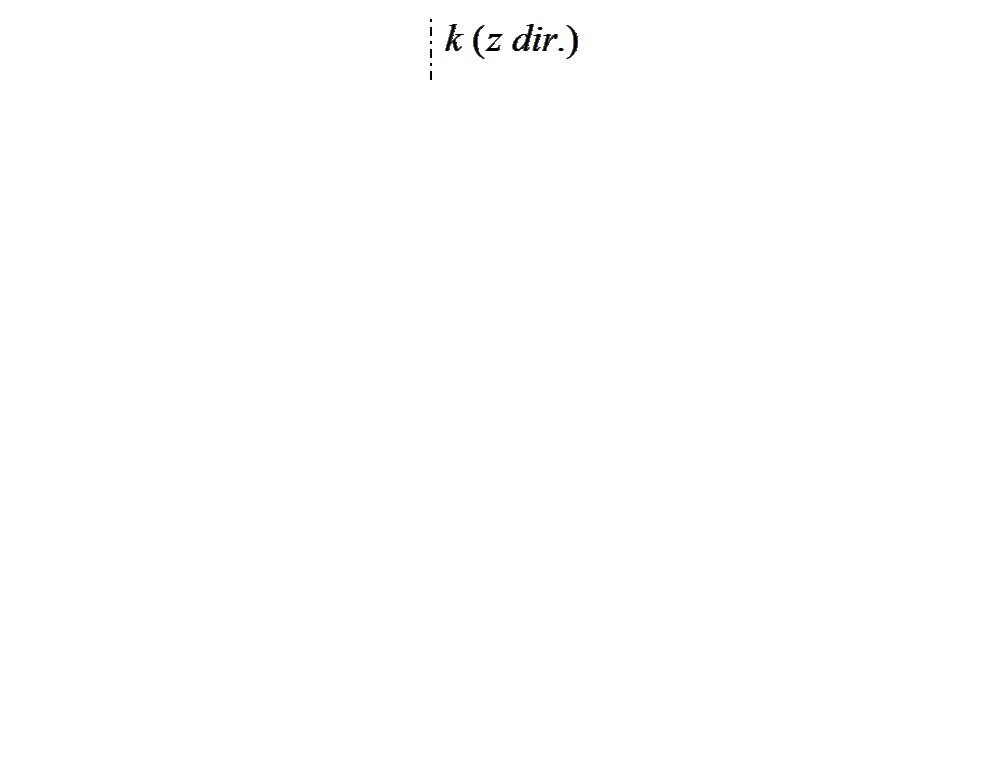
\includegraphics[scale=0.6]{./figure/cntrl-volume.eps}\\
    (b) Control volume for the momentum\\
  \includegraphics[scale=0.6]{./figure/cntrl-volume2.eps}\\
  \end{tabular}
\end{center}
  \caption{Control volume}
  \label{fig:cntrl-volume}
\end{figure}




\chapter{The physical parameterization}
%\documentclass{article}
%\usepackage{amsmath}
%\begin{document}

\section{Turbulence}
{\bf \Large
\begin{tabular}{ccc}
\hline
  Correnspoinding author & : & Seiya Nishizawa\\
\hline
\end{tabular}
}

\def\half{\frac{1}{2}}

\subsection{Spatial filter}

The governing euqations are the followings:
\begin{align}
  \frac{\partial\rho}{\partial t} + \frac{\partial u_i \rho}{\partial x_i}
  &= 0 \\
  \frac{\partial\rho u_i}{\partial t}
  + \frac{\partial u_j \rho u_i}{\partial x_j}
  &= -\frac{\partial p}{\partial x_i} + g \rho \delta_{i3} \\
  \frac{\partial\rho \theta}{\partial t}
  + \frac{\partial u_i \rho \theta}{\partial x_i}
  &= Q
\end{align}

Spatial filtering the continuity equation yields
\begin{equation}
  \frac{\partial \overline{\rho}}{\partial t} + \frac{\partial \overline{u_i \rho}}{\partial x_i} = 0, \label{eq: spatial filtered rho}
\end{equation}
where $\overline{\phi}$ means the spatial filtered quantity of an arbitrary variable $\phi$.
The Favre filtering \citep{Favre_1983} defined by
\begin{equation}
  \widetilde{\phi} = \frac{\overline{\rho \phi}}{\overline{\rho}}
\end{equation}
makes the equation (\ref{eq: spatial filtered rho})
\begin{equation}
  \frac{\partial \overline{\rho}}{\partial t} + \frac{\partial \widetilde{u_i}\overline{\rho}}{\partial x_i} = 0.
\end{equation}


The momentam equations become
\begin{align}
  \frac{\partial \overline{\rho u_i}}{\partial t} + \frac{\partial \overline{u_j\rho u_i}}{\partial x_j} &= -\frac{\partial \overline{p}}{\partial x_i} + \overline{\rho} g\delta_{i3} \\
  \frac{\partial \overline{\rho}\widetilde{u_i}}{\partial t} + \frac{\partial \widetilde{u_j}\:\overline{\rho}\widetilde{u_i}}{\partial x_j} &= -\frac{\partial \overline{p}}{\partial x_i} + g\overline{\rho} \delta_{i3}
    -\frac{\partial}{\partial x_j}\left(\overline{u_i \rho u_j} - \widetilde{u_j}\overline{\rho}\widetilde{u_i}\right) \\
  \frac{\partial \overline{\rho}\widetilde{u_i}}{\partial t} + \frac{\partial \widetilde{u_j}\:\overline{\rho}\widetilde{u_i}}{\partial x_j} &= -\frac{\partial \overline{p}}{\partial x_i} + g\overline{\rho} \delta_{i3}
    -\frac{\partial}{\partial x_j}\overline{\rho}\left(\widetilde{u_i u_j} - \widetilde{u_j}\widetilde{u_i}\right).
\end{align}


As the same matter, the thermal equation becomes
\begin{equation}
  \frac{\partial \overline{\rho}\widetilde{\theta}}{\partial t}
  + \frac{\partial \widetilde{u_i}\overline{\rho}\widetilde{\theta}}{\partial x_i}
  = Q -\frac{\partial}{\partial x_i}\overline{\rho}\left(\widetilde{u_i\theta}-\widetilde{u_i}\widetilde{\theta}\right).
\end{equation}

Then, the govering equations for the prognositic variables
($\overline{\rho}, \overline{\rho}\widetilde{u_i}, $ and $\overline{\rho}\widetilde{\theta}$) are
\begin{align}
  \frac{\partial \overline{\rho}}{\partial t}
  + \frac{\partial \widetilde{u_i}\overline{\rho}}{\partial x_i} &= 0, \\
  \frac{\partial \overline{\rho}\widetilde{u_i}}{\partial t}
  + \frac{\partial \widetilde{u_j}\overline{\rho}\widetilde{u_i}}{\partial x_j}
  &= -\frac{\partial \overline{p}}{\partial x_i} + g\overline{\rho}\delta_{i3}
  -\frac{\partial \overline{\rho}\tau_{ij}}{\partial x_j}, \\
  \frac{\partial \overline{\rho}\widetilde{\theta}}{\partial t}
  + \frac{\partial \widetilde{u_i}\overline{\rho}\widetilde{\theta}}{\partial x_i}
  &= Q -\frac{\partial \overline{\rho}\tau^D_{i}}{\partial x_i},
\end{align}
where
\begin{align}
  \tau_{ij} &= \widetilde{u_iu_j}-\widetilde{u_i}\widetilde{u_j}, \\
  \tau^D_{i} &= \widetilde{u_i\theta}-\widetilde{u_i}\widetilde{\theta}.
\end{align}

Hereafter, we omite overline and tilde representing spatial and the Favre filters.

\subsection{SGS model}
\subsubsection{Smagorinsky-Lilly model}
The eddy momentum flux is
\begin{equation}
  \tau_{ij} - \frac{1}{3}\tau_{kk}\delta_{ij} = -2\nu_{SGS}\left(S_{ij}-\frac{1}{3}S_{kk}\delta_{ij}\right),
\end{equation}
where $S_{ij}$ is the strain tensor,
\begin{equation}
  S_{ij} = \frac{1}{2}\left(\frac{\partial u_i}{\partial x_j} + \frac{\partial u_j}{\partial x_i}\right),
  \label{eq:strain tensor}
\end{equation}
and
\begin{equation}
  \nu_{SGS} = \left(C_s\lambda\right)^2 \left|S\right|.
\end{equation}
$C_s$ is the Smagorinsky constant,
$\lambda$ is a characteristic SGS length scale,
and $\left|S\right|$ is scale of the tensor $S$,
\begin{equation}
  \left|S\right| = \sqrt{2S_{ij}S_{ij}}.
  \label{eq:|S|}
\end{equation}

Then the eddy momentum flux is
\begin{equation}
  \tau_{ij} = -2\nu_{SGS}\left(S_{ij}-\frac{1}{3}S_{kk}\delta_{ij}\right)
             + \frac{2}{3} TKE\delta_{ij},
  \label{eq:tau}
\end{equation}
where
\begin{equation}
  TKE = \frac{1}{2}\tau_{ii}
   = \left(\frac{\nu_{SGS}}{C_k\lambda}\right)^2,
   \label{eq:tke}
\end{equation}
where $C_k$ is a SGS constant and assumed to be 0.1 by following \citet{Deardorff_1980} and \citet{Moeng_Wynggard_1988}.


The eddy heat flux is
\begin{equation}
  \tau^D_i = -D_{SGS} \frac{\partial \theta}{\partial x_i},
  \label{eq:tau*}
\end{equation}
where
\begin{equation}
  D_{SGS} = \frac{1}{Pr}\nu_{SGS}.
\end{equation}
$Pr$ is the turbulent Prandtl number.
For the other scalar constants such as water vaper,
$D_{SGS}$ is also used as their diffusivity.

To include buoyancy effects,
the extension of the basic Smagorinsky developed by \citet{Brown_etal_1994}
is used.
\begin{equation}
  \nu_{SGS} = (C_s\lambda)^2 |S| \sqrt{1-Rf},
\end{equation}
where $Rf$ is the flux Richardson number ($Rf = Ri/Pr$).
$Ri$ is the local (pointwise) gradient Richardson number,
\begin{equation}
  Ri = \frac{N^2}{|S|^2},
  \label{eq:Ri}
\end{equation}
and $N^2$ is the Brunt-Visala frequency,
\begin{equation}
  N^2 = \frac{g}{\theta}\frac{\partial\theta}{\partial z}.
  \label{eq:N^2}
\end{equation}
The Prandtl number is an unknow parameter,
and it depends on the Richardson number,
while it is offten assumed a constant value.
For the unstable conditions ($Ri < 0$),
\begin{align}
  \nu_{SGS} &= \left(C_s\lambda\right)^2 |S| \sqrt{1 - c Ri}, \label{eq:nu unstable} \\
  D_{SGS} &= \frac{1}{Pr_N} \left(C_s\lambda\right)^2 |S| \sqrt{1 - b Ri} \label{eq:nu^* unstable},
\end{align}
where $Pr_N$ is the Prandtl number in neutral condtions.
The values of $c, b, Pr_N$ are set 16, 40, and 0.7, respectively.
Then the Prandtl number is
\begin{equation}
  Pr = Pr_N \sqrt{\frac{1-c Ri}{1-b Ri}}.
\end{equation}
For the stable condtions,
when the Richardson number is smaller than the critical Richardson number, $Ri_c (=0.25)$,
\begin{align}
  \nu_{SGS} &= \left(C_s\lambda\right)^2 |S| \left(1-\frac{Ri}{Ri_c}\right)^4, \label{eq:nu stable} \\
  D_{SGS} &= \frac{1}{Pr_N}\left(C_s\lambda\right)^2 |S| \left(1-\frac{Ri}{Ri_c}\right)^4\left(1-g Ri\right). \label{eq:nu^* stable}
\end{align}
The constant $g$ is determined as the Prandtl number becomes 1
in the limit of $Ri \to Ri_C$ and then is $(1-Pr_N)/Ri_c$.
The Prandtl number is
\begin{equation}
  Pr = Pr_N \left\{1-(1-Pr_N)\frac{Ri}{Ri_c}\right\}^{-1}.
\end{equation}
For the strongly stable condistions ($Ri > Ri_c$),
the eddy viscosity and the diffusivity for scalars are 0;
\begin{align}
  \nu_{SGS} &= 0, \label{eq:nu strong stable} \\
  D_{SGS} &= 0. \label{eq:nu^* strong stable}
\end{align}
The Prandtl number is $Pr = 1$.


\citet{Scotti_1993} suggested that the length scale should depend on the grid aspect ratio.
In the equilibrium condition with the universal Kolmogorov spectrum, energy cascaded to the SGS turbulence, which equals to SGS dissipation, must not depend on grid aspect ratio.
The energy flux or dissipation can be written as function of $S_{ij}$ and the length scale, $\lambda$.
The $S_{ij}$ depends on the grid aspect ratio, so the length scale should have dependency on the aspect ratio which cancels the dependency of the $S_{ij}$.
With some approximations, they obtained an approximate function of the length scale
\footnote{They considered two grid aspect ratios, while we here think only one, i.e. $\Delta x = \Delta y$.}
:
\begin{equation}
\lambda = f(a) \Delta,
\end{equation}
%\begin{equation}
%  \frac{1}{\lambda^2} = \frac{1}{\lambda_0^2} + \frac{1}{(kz)^2},
%\end{equation}
%where $k$ is the Karman constant ($k=0.4$), and $\lambda_0 = f(a) \Delta$.
where $f(a)$ is a function of grid aspect ratio, $a$, and
\begin{align}
  f(a) &= 1.736 a^{1/3} \{ \nonumber\\
  & 4P_1(b_1)a^{1/3} + 0.222P_2(b_1)a^{-5/3} + 0.077P_3(b_1)a^{-11/3} \nonumber\\
  & - 3b_1 + 4P_1(b_2) + 0.222P_2(b_2) + 0.077P_3(b_2)- 3b_2 \nonumber\\
  & \}^{-3/4}. \label{eq: f}
\end{align}
Here $b_1 = \arctan(1/a), b_2 = \arctan(a) = \pi/2 - b_1$, and
\begin{align}
  P_1(z) &= 2.5P_2(z) - 1.5 (\cos(z))^{2/3} \sin(z), \\
  P_2(z) &= 0.98z + 0.073z^2 -0.418z^3 + 0.120z^4, \\
  P_3(z) &= 0.976z + 0.188z^2 + 1.169z^3 + 0.755z^4 - 0.151z^5.
\end{align}
For instance, $f(2) = 1.036, f(5) = 1.231, f(10) = 1.469$, and $f(20) = 1.790$.
%For instance, $f(2) = 1.036, f(5) = 1.231, f(10) = 1.469, f(20) = 1.790$, and $f(50) = 2.368$.
$\Delta$ is the filter length, and is defined to be proportional to $(\Delta x \Delta y \Delta z)^{1/3}$ here.
In this model, we introduce a numerical filter to reduce two-grid noise discussed above.
This filter reduces two-grid scale physical variability as well.
This means that two-grid scale would be preferred for the filter length in this model rather than grid spacing itself, that is,
\begin{equation}
  \Delta = 2 (\Delta x \Delta y \Delta z)^{1/3}. \label{eq: delta}
\end{equation}


\subsubsection{Terrain-following coordinate}
Tendencies representing effect of the sub-grid scale turbulence with the terrain-following coordinate are following
\footnote{Equations which are not changed in the terrain-following coordinate are ommited.};
\begin{align}
  \frac{\partial G^{\frac{1}{2}}\rho u}{\partial t}
  &=
  - \frac{\partial G^{\frac{1}{2}}\rho\tau_{11}}{\partial x^*}
  - \frac{\partial G^{\frac{1}{2}}\rho\tau_{12}}{\partial y^*}
  - \frac{\partial J_{13}G^{\frac{1}{2}}\rho\tau_{11} + J_{23}G^{\frac{1}{2}}\rho\tau_{12} + J_{33}G^{\frac{1}{2}}\rho\tau_{13}}{\partial \xi}, \\
  \frac{\partial G^{\frac{1}{2}}\rho v}{\partial t}
  &=
  - \frac{\partial G^{\frac{1}{2}}\rho\tau_{21}}{\partial x^*}
  - \frac{\partial G^{\frac{1}{2}}\rho\tau_{22}}{\partial y^*}
  - \frac{\partial J_{13}G^{\frac{1}{2}}\rho\tau_{21} + J_{23}G^{\frac{1}{2}}\rho\tau_{22} + J_{33}G^{\frac{1}{2}}\rho\tau_{23}}{\partial \xi}, \\
  \frac{\partial G^{\frac{1}{2}}\rho w}{\partial t}
  &=
  - \frac{\partial G^{\frac{1}{2}}\rho\tau_{31}}{\partial x^*}
  - \frac{\partial G^{\frac{1}{2}}\rho\tau_{32}}{\partial y^*}
  - \frac{\partial J_{13}G^{\frac{1}{2}}\rho\tau_{31} + J_{23}G^{\frac{1}{2}}\rho\tau_{32} + J_{33}G^{\frac{1}{2}}\rho\tau_{33}}{\partial \xi}, \\
  \frac{\partial G^{\frac{1}{2}} \rho \theta}{\partial t}
  &=
  - \frac{\partial G^{\frac{1}{2}}\rho\tau^D_1}{\partial x^*}
  - \frac{\partial G^{\frac{1}{2}}\rho\tau^D_2}{\partial y^*}
  - \frac{\partial J_{13}G^{\frac{1}{2}}\rho\tau^D_1 + J_{23}G^{\frac{1}{2}}\rho\tau^D_2 + J_{33}G^{\frac{1}{2}}\rho\tau^D_3}{\partial \xi}
\end{align}
\begin{align}
  G^{\frac{1}{2}}S_{11} &= \frac{\partial G^{\frac{1}{2}}u}{\partial x^*} + \frac{\partial J_{13}G^{\frac{1}{2}}u}{\partial \xi}, \\
  G^{\frac{1}{2}}S_{22} &= \frac{\partial G^{\frac{1}{2}}v}{\partial y^*} + \frac{\partial J_{23}G^{\frac{1}{2}}v}{\partial \xi}, \\
  G^{\frac{1}{2}}S_{33} &= \frac{\partial J_{33}G^{\frac{1}{2}}w}{\partial \xi}, \\
  G^{\frac{1}{2}}S_{12} &= \frac{1}{2}\left(\frac{\partial G^{\frac{1}{2}}u}{\partial y^*} + \frac{\partial G^{\frac{1}{2}}v}{\partial x^*} + \frac{\partial J_{23}G^{\frac{1}{2}}u + J_{13}G^{\frac{1}{2}}v}{\partial \xi}\right), \\
  G^{\frac{1}{2}}S_{23} &= \frac{1}{2}\left(\frac{\partial G^{\frac{1}{2}}w}{\partial y^*} + \frac{\partial J_{33}G^{\frac{1}{2}}v + J_{23}G^{\frac{1}{2}}w}{\partial \xi}\right), \\
  G^{\frac{1}{2}}S_{31} &= \frac{1}{2}\left(\frac{\partial G^{\frac{1}{2}}w}{\partial x^*} + \frac{\partial J_{13}G^{\frac{1}{2}}w + J_{33}G^{\frac{1}{2}}u}{\partial \xi}\right), \\
  G^{\frac{1}{2}}\tau^D_1 &= -D_{SGS}\left(
   \frac{\partial G^{\frac{1}{2}}\theta}{\partial x^*}
  +\frac{\partial J_{13}G^{\frac{1}{2}}\theta}{\partial \xi} \right), \\
  G^{\frac{1}{2}}\tau^D_2 &= -D_{SGS}\left(
   \frac{\partial G^{\frac{1}{2}}\theta}{\partial y^*}
  +\frac{\partial J_{23}G^{\frac{1}{2}}\theta}{\partial \xi} \right), \\
  G^{\frac{1}{2}}\tau^D_3 &= -D_{SGS}
  \frac{\partial J_{33}G^{\frac{1}{2}}\theta}{\partial \xi}, \\
  G^{\frac{1}{2}} N^2 &= \frac{g}{\theta}\frac{\partial J_{33}G^{\frac{1}{2}}\theta}{\partial \xi}.
\end{align}



\subsection{descretization}

\subsubsection{Spatial descretization}
We use the 4th order differnce scheme for the advection term as mentioned
in the chapter \ref{chap:descretization dynamics}.
The $\tau_{ij}$ and $\tau^D_{i}$ are propotional to
the square of the grid spacing ($\Delta^2$).
Due to the consistency with the advection term
in terms of order for spatial difference,
the second order central difference scheme
is used for terms of the sub-grid scale turburence.
In the following part in this sub-section,
overline, and $i,j,k$ mean
as they are in the chapter \ref{chap:descretization dynamics}.

\paragraph{Momentam equation}
The tendencies in the momentam equation related to the sub-grid scale mode are
\begin{align}
  \frac{\partial G^{\frac{1}{2}}\rho u}{\partial t}_{i+\half,j,k} =
  &-\frac{(G^{\frac{1}{2}}\rho\tau_{11})_{i+1,j,k}-(G^{\frac{1}{2}}\rho\tau_{11})_{i,j,k}}{\Delta x} \nonumber \\
  &- \frac{(G^{\frac{1}{2}}\overline{\rho}\tau_{12})_{i+\half,j+\half,k}-(G^{\frac{1}{2}}\overline{\rho}\tau_{12})_{i+\half,j-\half,k}}{\Delta y} \nonumber \\
  &- \frac{\{G^{\frac{1}{2}}\overline{\rho}(J_{13}\tau_{11}+J_{23}\tau_{12}+J_{33}\tau_{13})\}_{i+\half,j,k+\half}
          -\{G^{\frac{1}{2}}\overline{\rho}(J_{13}\tau_{11}+J_{23}\tau_{12}+J_{33}\tau_{13})\}_{i+\half,j,k-\half}}{\Delta z}, \\
  \frac{\partial G^{\frac{1}{2}}\rho v}{\partial t}_{i,j+\half,k} =
  &- \frac{(G^{\frac{1}{2}}\overline{\rho}\tau_{21})_{i+\half,j+\half,k}-(G^{\frac{1}{2}}\overline{\rho}\tau_{21})_{i-\half,j+\half,k}}{\Delta x} \nonumber \\
  &- \frac{(G^{\frac{1}{2}}\rho\tau_{22})_{i,j+1,k}-(G^{\frac{1}{2}}\rho\tau_{22})_{i,j,k}}{\Delta y} \nonumber \\
  &- \frac{\{G^{\frac{1}{2}}\overline{\rho}(J_{13}\tau_{21}+J_{23}\tau_{22}+J_{33}\tau_{23})\}_{i,j+\half,k+\half}
          -\{G^{\frac{1}{2}}\overline{\rho}(J_{13}\tau_{21}+J_{23}\tau_{22}+J_{33}\tau_{23})\}_{i,j+\half,k-\half}}{\Delta z}, \\
  \frac{\partial G^{\frac{1}{2}}\rho w}{\partial t}_{i,j,k+\half} =
  &- \frac{(G^{\frac{1}{2}}\overline{\rho}\tau_{31})_{i+\half,j,k+\half}-(G^{\frac{1}{2}}\overline{\rho}\tau_{31})_{i-\half,j,k+\half}}{\Delta x} \nonumber \\
  &- \frac{(G^{\frac{1}{2}}\overline{\rho}\tau_{32})_{i,j+\half,k+\half}-(G^{\frac{1}{2}}\overline{\rho}\tau_{32})_{i,j-\half,k+\half}}{\Delta y} \nonumber \\
  &- \frac{\{(G^{\frac{1}{2}}\rho(J_{13}\tau_{31}+J_{23}\tau_{32}+J_{33}\tau_{33})\}_{i,j,k+1}
          -\{(G^{\frac{1}{2}}\rho(J_{13}\tau_{31}+J_{23}\tau_{32}+J_{33}\tau_{33})\}_{i,j,k}}{\Delta z}.
\end{align}
The $\overline{\rho}$ is
\begin{align}
  \overline{\rho}_{i,j+\half,k+\half} &=
  \frac{\rho_{i,j+1,k+1} + \rho_{i,j+1,k} + \rho_{i,j,k+1} + \rho_{i,j,k}}{4}, \\
  \overline{\rho}_{i+\half,j,k+\half} &=
  \frac{\rho_{i+1,j,k+1} + \rho_{i+1,j,k} + \rho_{i,j,k+1} + \rho_{i,j,k}}{4}, \\
  \overline{\rho}_{i+\half,j+\half,k} &=
  \frac{\rho_{i+1,j+1,k} + \rho_{i+1,j,k} + \rho_{i,j+1,k} + \rho_{i,j,k}}{4}.
\end{align}

\paragraph{Thermal equation}
The tendency in the thermal equation related to the sub-grid scale model is
\begin{align}
  \frac{\partial G^{\frac{1}{2}}\rho \theta}{\partial t}_{i,j,k} =
  &- \frac{(G^{\frac{1}{2}}\overline{\rho}\tau^D_1)_{i+\half,j,k}-(G^{\frac{1}{2}}\overline{\rho}\tau^D_1)_{i-\half,j,k}}{\Delta x} \nonumber \\
  &- \frac{(G^{\frac{1}{2}}\overline{\rho}\tau^D_2)_{i,j+\half,k}-(G^{\frac{1}{2}}\overline{\rho}\tau^D_2)_{i,j-\half,k}}{\Delta y} \nonumber \\
  &- \frac{\{G^{\frac{1}{2}}\overline{\rho}(J_{13}\tau^D_1+J_{23}\tau^D_2+J_{33}\tau^D_3)\}_{i,j,k+\half}
          -\{G^{\frac{1}{2}}\overline{\rho}(J_{13}\tau^D_1+J_{23}\tau^D_2+J_{33}\tau^D_3)\}_{i,j,k-\half}}{\Delta z}.
\end{align}
The $\overline{\rho}$ at half-level is eq.(\ref{eq:rho half i})-(\ref{eq:rho half k}).

The eddy diffution flux, $\tau^D$, at half-level
is
\begin{align}
  (G^{\frac{1}{2}}\tau^D_1)_{i+\half,j,k} &= -D_{SGS,i+\half,j,k} \left\{
  \frac{(G^{\frac{1}{2}}\theta)_{i+1,j,k}-(G^{\frac{1}{2}}\theta)_{i,j,k}}{\Delta x}
  + \frac{(J_{13}G^{\frac{1}{2}}\overline{\theta})_{i+\half,j,k+\half}-(J_{13}G^{\frac{1}{2}}\overline{\theta})_{i+\half,j,k-\half}}{\Delta z} \right\}, \\
  (G^{\frac{1}{2}}\tau^D_2)_{i,j+\half,k} &= -D_{SGS,i,j+\half,k} \left\{
  \frac{(G^{\frac{1}{2}}\theta)_{i,j+1,k}-(G^{\frac{1}{2}}\theta)_{i,j,k}}{\Delta y}
  + \frac{(J_{23}G^{\frac{1}{2}}\overline{\theta})_{i,j+\half,k+\half}-(J_{23}G^{\frac{1}{2}}\overline{\theta})_{i,j+\half,k-\half}}{\Delta z} \right\}, \\
  (G^{\frac{1}{2}}\tau^D_3)_{i,j,k+\half} &= -D_{SGS,i,j,k+\half} \frac{J_{33}G^{\frac{1}{2}}\theta_{i,j,k+1}-J_{33}G^{\frac{1}{2}}\theta_{i,j,k}}{\Delta z}.
\end{align}



\paragraph{Strain tensor}
All the strain tensor, eq.(\ref{eq:strain tensor}), have to be calculated
at full-level (grid cell center),
and some of them are at cell edges.

\begin{itemize}
  \item cell center ($i,j,k$)
    \begin{align}
      (G^{\frac{1}{2}}S_{11})_{i,j,k} &=
      \frac{(G^{\frac{1}{2}}\overline{u})_{i+\half,j,k}-(G^{\frac{1}{2}}\overline{u})_{i-\half,j,k}}{\Delta x}
     +\frac{(J_{13}G^{\frac{1}{2}}\overline{u})_{i+\half,j,k+\half}-(J_{13}G^{\frac{1}{2}}\overline{u})_{i+\half,j,k-\half}}{\Delta z}, \\
     (G^{\frac{1}{2}}S_{22})_{i,j,k} &=
      \frac{(G^{\frac{1}{2}}\overline{v})_{i,j+\half,k}-(G^{\frac{1}{2}}\overline{v})_{i,j-\half,k}}{\Delta y}
     +\frac{(J_{23}G^{\frac{1}{2}}\overline{v})_{i,j+\half,k+\half}-(J_{23}G^{\frac{1}{2}}\overline{v})_{i,j+\half,k-\half}}{\Delta z}, \\
     (G^{\frac{1}{2}}S_{33})_{i,j,k} &=
      \frac{J_{33}G^{\frac{1}{2}}\overline{w}_{i,j,k+\frac{1}{2}}-J_{33}G^{\frac{1}{2}}\overline{w}_{i,j,k-\frac{1}{2}}}{\Delta z}, \\
      (G^{\frac{1}{2}}S_{12})_{i,j,k} &= \frac{1}{2}\left\{
      \frac{(G^{\frac{1}{2}}\overline{u})_{i,j+\frac{1}{2},k}-(G^{\frac{1}{2}}\overline{u})_{i,j-\frac{1}{2},k}}{\Delta y}
     +\frac{(G^{\frac{1}{2}}\overline{v})_{i+\frac{1}{2},j,k}-(G^{\frac{1}{2}}\overline{v})_{i-\frac{1}{2},j,k}}{\Delta x}  \right.\nonumber \\ &\left.
     +\frac{(J_{23}G^{\frac{1}{2}}\overline{u})_{i,j,k+\half}-(J_{23}G^{\frac{1}{2}}\overline{u})_{i,j,k-\half} + (J_{13}G^{\frac{1}{2}}\overline{v})_{i,j,k+\half}-(J_{13}G^{\frac{1}{2}}\overline{v})_{i,j,k-\half}}{\Delta z}
      \right\}, \\
      (G^{\frac{1}{2}}S_{23})_{i,j,k} &= \frac{1}{2}\left\{
      \frac{(G^{\frac{1}{2}}\overline{w})_{i,j+\frac{1}{2},k}-(G^{\frac{1}{2}}\overline{w})_{i,j-\frac{1}{2},k}}{\Delta y} \right. \nonumber \\ & \left.
      + \frac{J_{33}G^{\frac{1}{2}}\overline{v}_{i,j,k+\frac{1}{2}}-J_{33}G^{\frac{1}{2}}\overline{v}_{i,j,k-\frac{1}{2}} + (J_{23}G^{\frac{1}{2}}\overline{w})_{i,j,k+\half}-(J_{23}G^{\frac{1}{2}}\overline{w})_{i,j,k-\half}}{\Delta z}
      \right\}, \\
      (G^{\frac{1}{2}}S_{31})_{i,j,k} &= \frac{1}{2}\left\{
      \frac{(G^{\frac{1}{2}}\overline{w})_{i+\frac{1}{2},j,k}-(G^{\frac{1}{2}}\overline{w})_{i-\frac{1}{2},j,k}}{\Delta x} \right. \nonumber \\ & \left.
     +\frac{J_{33}G^{\frac{1}{2}}\overline{u}_{i,j,k+\frac{1}{2}}-J_{33}G^{\frac{1}{2}}\overline{u}_{i,j,k-\frac{1}{2}} + (J_{13}G^{\frac{1}{2}}\overline{w})_{i,j,k+\half}-(J_{13}G^{\frac{1}{2}}\overline{w})_{i,j,k-\half}}{\Delta z}
      \right\}.
    \end{align}

  \item $z$ edge ($i+\half,j+\half,k$)
    \begin{align}
      (G^{\frac{1}{2}}S_{12})_{i+\half,j+\half,k} &= \frac{1}{2}\left\{
      \frac{(G^{\frac{1}{2}}\overline{u})_{i+\half,j+1,k}-(G^{\frac{1}{2}}\overline{u})_{i+\half,j,k}}{\Delta y}
     +\frac{(G^{\frac{1}{2}}\overline{v})_{i+1,j+\half,k}-(G^{\frac{1}{2}}\overline{v})_{i,j+\half,k}}{\Delta x}  \right.\nonumber \\ &\left.
     +\frac{(J_{23}G^{\frac{1}{2}}\overline{u})_{i+\half,j+\half,k+\half}-(J_{23}G^{\frac{1}{2}}\overline{u})_{i+\half,j+\half,k-\half} + (J_{13}G^{\frac{1}{2}}\overline{v})_{i+\half,j+\half,k+\half}-(J_{13}G^{\frac{1}{2}}\overline{v})_{i+\half,j+\half,k-\half}}{\Delta z}.
      \right\}
    \end{align}

  \item $x$ edge ($i,j+\half,k+\half$)
    \begin{align}
      (G^{\frac{1}{2}}S_{23})_{i,j+\half,k+\half} &= \frac{1}{2}\left\{
      \frac{(G^{\frac{1}{2}}\overline{w})_{i,j+1,k+\half}-(G^{\frac{1}{2}}\overline{w})_{i,j,k+\half}}{\Delta y} \right. \nonumber \\ & \left.
      + \frac{J_{33}G^{\frac{1}{2}}\overline{v}_{i,j+\half,k+1}-J_{33}G^{\frac{1}{2}}\overline{v}_{i,j+\half,k} + (J_{23}G^{\frac{1}{2}}\overline{w})_{i,j+\half,k+1}-(J_{23}G^{\frac{1}{2}}\overline{w})_{i,j+\half,k}}{\Delta z}.
      \right\}
    \end{align}

  \item $y$ edge ($i+\half,j,k+\half$)
    \begin{align}
      (G^{\frac{1}{2}}S_{31})_{i+\half,j,k+\half} &= \frac{1}{2}\left\{
      \frac{(G^{\frac{1}{2}}\overline{w})_{i+1,j,k+\half}-(G^{\frac{1}{2}}\overline{w})_{i,j,k+\half}}{\Delta x} \right. \nonumber \\ & \left.
     +\frac{J_{33}G^{\frac{1}{2}}\overline{u}_{i+\half,j,k+1}-J_{33}G^{\frac{1}{2}}\overline{u}_{i+\half,j,k} + (J_{13}G^{\frac{1}{2}}\overline{w})_{i+\half,j,k+1}-(J_{13}G^{\frac{1}{2}}\overline{w})_{i+\half,j,k}}{\Delta z}.
      \right\}.
    \end{align}

\end{itemize}


\paragraph{velocity}
Calculattion of the strain tensor
requires value of velocity
at cell center, plane center, edge center, and vertex.
The velocities at cell center (full-level) are eq.(\ref{eq:u full}-\ref{eq:w full}).

\begin{itemize}
  \item $x$-$y$ plane center ($i,j,k+\frac{1}{2}$)
    \begin{align}
      \overline{u}_{i,j,k+\frac{1}{2}} &=
      \frac{\overline{u}_{i,j,k+1}+\overline{u}_{i,j,k}}{2}, \\
      \overline{v}_{i,j,k+\frac{1}{2}} &=
      \frac{\overline{v}_{i,j,k+1}+\overline{v}_{i,j,k}}{2}, \\
      \overline{w}_{i,j,k+\frac{1}{2}} &=
      \frac{(\rho w)_{i,j,k+\frac{1}{2}}}{\overline{\rho}_{i,j,k+\frac{1}{2}}}.
    \end{align}

  \item $y$-$z$ plane center ($i+\frac{1}{2},j,k$)
    \begin{align}
      \overline{u}_{i+\frac{1}{2},j,k} &=
      \frac{(\rho u)_{i+\frac{1}{2},j,k}}{\overline{\rho}_{i+\frac{1}{2},j,k}}, \\
      \overline{v}_{i+\frac{1}{2},j,k} &=
      \frac{\overline{v}_{i+1,j,k}+\overline{v}_{i,j,k}}{2}, \\
      \overline{w}_{i+\frac{1}{2},j,k} &=
      \frac{\overline{w}_{i+1,j,k}+\overline{w}_{i,j,k}}{2}.
    \end{align}

  \item $z$-$x$ plane center ($i,j+\frac{1}{2},k$)
    \begin{align}
      \overline{u}_{i,j+\frac{1}{2},k} &=
      \frac{\overline{u}_{i,j+1,k}+\overline{u}_{i,j,k}}{2}, \\
      \overline{v}_{i,j+\frac{1}{2},k} &=
      \frac{(\rho v)_{i,j+\frac{1}{2},k}}{\overline{\rho}_{i,j+\frac{1}{2},k}}, \\
      \overline{w}_{i,j+\frac{1}{2},k} &=
      \frac{\overline{w}_{i,j+1,k}+\overline{w}_{i,j,k}}{2}.
    \end{align}

  \item $x$ edge center ($i,j+\frac{1}{2},k+\half$)
    \begin{align}
      \overline{u}_{i,j+\half,k+\half} &=
      \frac{\overline{u}_{i,j+1,k+1}+\overline{u}_{i,j+1,k}+\overline{u}_{i,j,k+1}+\overline{u}_{i,j,k}}{4}, \\
      \overline{v}_{i,j+\half,k+\half} &=
      \frac{\overline{v}_{i,j+\half,k+1}+\overline{v}_{i,j+\half,k}}{2}, \\
      \overline{w}_{i,j+\half,k+\half} &=
      \frac{\overline{w}_{i,j+1,k+\half}+\overline{w}_{i,j,k+\half}}{2}.
    \end{align}

  \item $y$ edge center ($i+\half,j,k+\half$)
    \begin{align}
      \overline{u}_{i+\half,j,k+\half} &=
      \frac{\overline{u}_{i+\half,j,k+1}+\overline{u}_{i+\half,j,k}}{2}, \\
      \overline{v}_{i+\half,j,k+\half} &=
      \frac{\overline{v}_{i+1,j,k+1}+\overline{v}_{i+1,j,k}+\overline{v}_{i,j,k+1}+\overline{v}_{i,j,k}}{4}, \\
      \overline{w}_{i+\half,j,k+\half} &=
      \frac{\overline{w}_{i+1,j,k+\half}+\overline{w}_{i,j,k+\half}}{2}.
    \end{align}

  \item $z$ edge center ($i+\half,j+\half,k$)
    \begin{align}
      \overline{u}_{i+\half,j+\half,k} &=
      \frac{\overline{u}_{i+\half,j+1,k}+\overline{u}_{i+\half,j,k}}{2}, \\
      \overline{v}_{i+\half,j+\half,k} &=
      \frac{\overline{v}_{i+1,j+\half,k}+\overline{v}_{i,j+\half,k}}{2}, \\
      \overline{w}_{i+\half,j+\half,k} &=
      \frac{\overline{w}_{i+1,j+1,k}+\overline{w}_{i+1,j,k}+\overline{w}_{i,j+1,k}+\overline{w}_{i,j,k}}{4}.
    \end{align}

  \item vertex ($i+\half,j+\half,k+\half$)
    \begin{align}
      \overline{u}_{i+\half,j+\half,k+\half} &=
      \frac{\overline{u}_{i+\half,j+1,k+1}+\overline{u}_{i+\half,j+1,k}+\overline{u}_{i+\half,j,k+1}+\overline{u}_{i+\half,j,k}}{4}, \\
      \overline{v}_{i+\half,j+\half,k+\half} &=
      \frac{\overline{v}_{i+1,j+\half,k+1}+\overline{v}_{i+1,j+\half,k}+\overline{v}_{i,j+\half,k+1}+\overline{v}_{i,j+\half,k}}{4}, \\
      \overline{w}_{i+\half,j+\half,k+\half} &=
      \frac{\overline{w}_{i+1,j+1,k+\half}+\overline{w}_{i+1,j,k+\half}+\overline{w}_{i,j+1,k+\half}+\overline{w}_{i,j,k+\half}}{4}.
    \end{align}
\end{itemize}

\paragraph{Eddy viscosity/diffusion coefficient}
The eddy viscosity/diffusion coefficient, $\nu_{SGS}$ / $D_{SGS}$, is calculated at full-level with $S$ and $Ri$ at full-level and it at half level is interporated one at full-level.


\paragraph{Brunt-Visala frequency}
The Brunt-Visala frequency, $N^2$ is required to calculate the Richardson number
at full-level.

\begin{equation}
  (G^{\half}N^2)_{i,j,k} = \frac{g}{\theta_{i,j,k}}
  \frac{J_{33}G^{\half}\theta_{i,j,k+1}-J_{33}G^{\half}\theta_{i,j,k-1}}{2\Delta z}.
\end{equation}



%\end{document}


\section{Microphysics}
{\Huge TBD}

\section{Radiation}
{\Huge TBD}

\section{Surface flux}
{\Huge TBD}




\appendix

\chapter{4th order central differnce}
{
\footnotesize
The 4th order central difference is given by
\begin{eqnarray}
&& \frac{\partial \phi}{\partial x}
=\frac{-\phi_{i+2}+8\phi_{i+1}-8\phi_{i-1}+\phi_{i+2}}{12\Delta x} = 0
\end{eqnarray}
where
\begin{eqnarray}
&& \phi_{i+2} = \phi_{i}
+ 2 \Delta x \left(\frac{\partial \phi}{\partial x}\right)_{i}
+ 2 \Delta x^2 \left(\frac{\partial^2 \phi}{\partial x^2}\right)_{i}
+ \frac{4 \Delta x^3}{3} \left(\frac{\partial^3 \phi}{\partial x^3}\right)_{i}
+ \frac{2 \Delta x^4}{3} \left(\frac{\partial^3 \phi}{\partial x^4}\right)_{i}
+ O(\Delta x^5)\\
&& \phi_{i+1} = \phi_{i}
+ \Delta x \left(\frac{\partial \phi}{\partial x}\right)_{i}
+ \frac{\Delta x^2}{2} \left(\frac{\partial^2 \phi}{\partial x^2}\right)_{i}
+ \frac{\Delta x^3}{6} \left(\frac{\partial^3 \phi}{\partial x^3}\right)_{i}
+ \frac{\Delta x^4}{24} \left(\frac{\partial^3 \phi}{\partial x^4}\right)_{i}
+ O(\Delta x^5)\\
&& \phi_i = \phi_i\\
&& \phi_{i-1} = \phi_{i}
- \Delta x \left(\frac{\partial \phi}{\partial x}\right)_{i}
+ \frac{\Delta x^2}{2} \left(\frac{\partial^2 \phi}{\partial x^2}\right)_{i}
- \frac{\Delta x^3}{6} \left(\frac{\partial^3 \phi}{\partial x^3}\right)_{i}
+ \frac{\Delta x^4}{24} \left(\frac{\partial^3 \phi}{\partial x^4}\right)_{i}
+ O(\Delta x^5)\\
&& \phi_{i+2} = \phi_{i}
- 2 \Delta x \left(\frac{\partial \phi}{\partial x}\right)_{i}
+ 2 \Delta x^2 \left(\frac{\partial^2 \phi}{\partial x^2}\right)_{i}
- \frac{4 \Delta x^3}{3} \left(\frac{\partial^3 \phi}{\partial x^3}\right)_{i}
+ \frac{2 \Delta x^4}{3} \left(\frac{\partial^3 \phi}{\partial x^4}\right)_{i}
+ O(\Delta x^5)
\end{eqnarray}
Therefore,
\begin{eqnarray}
&&
\frac{-\phi_{i+2}+8\phi_{i+1}-8\phi_{i-1}+\phi_{i+2}}{12\Delta x}
= \left(\frac{\partial \phi}{\partial x}\right)_{i}+ O(\Delta x^4)\\
&&
\frac{(-\phi_{i+2}+7\phi_{i+1}+7\phi_{i}-\phi_{i-1})-
(-\phi_{i+1}+7\phi_{i}+7\phi_{i-1}-\phi_{i-2})}{12\Delta x}
= \left(\frac{\partial \phi}{\partial x}\right)_{i}+ O(\Delta x^4)
\end{eqnarray}




\begin{figure}[t]
  (a)\\
  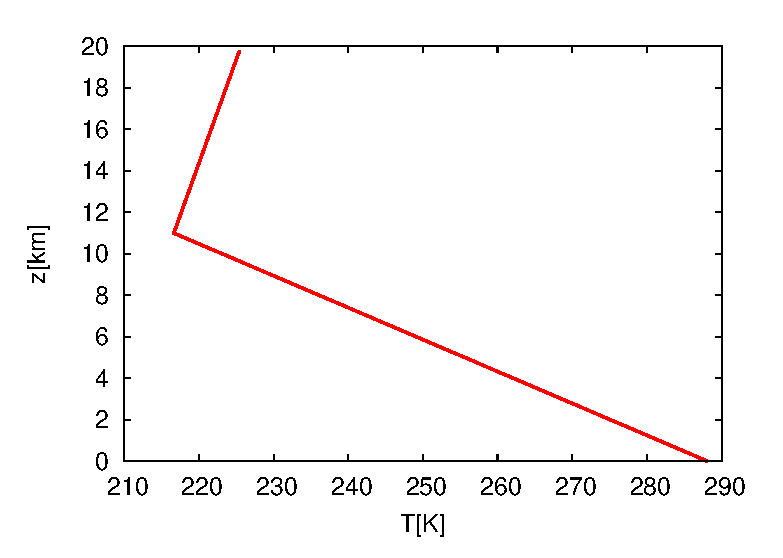
\includegraphics{b.eps}\\
  (b)\\
  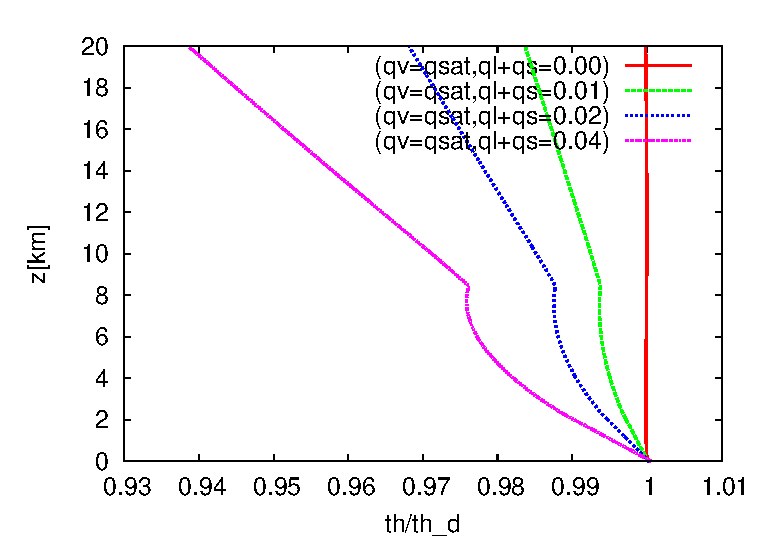
\includegraphics{a.eps}\\
  \caption{Thee vertical profile of (a) U.S. standard atmosphere,
  (b) the $\alpha$s.}
  \label{fig:fig1}
\end{figure}

\begin{table}[p]
  \caption{Notation of symbols}
  \begin{tabular}{lll}\hline
    $\rho$ & total density                       &  $kg/m^3$\\
    $q_d$  & mass concentration of dry air       &  $-$   \\
    $q_v$  & mass concentration of water vapor   &  $-$   \\
    $q_l$  & mass concentration of liquid water &   $-$   \\
    $q_s$  & mass concentration of solid water &    $-$   \\
    $t$    & time                              &   $s$   \\
    ${\bf u}$  & velocity of air flow          &   $m/s$   \\
    $w_l$  & relative velocity of liquid water to the gas    &   $m/s$   \\
    $w_s$  & relative velocity of solid water to the gas    &    $m/s$   \\
    ${\rm DIFF}\left[ x \right]$  & Diffusion term by turbulene  &    $kg/m^3\left[x\right]/s$   \\
    $S_v$    & source term of water vapor                     &    $kg/m^3/s$   \\
    $S_l$    & source term of liquid water                     &   $kg/m^3/s$   \\
    $S_s$    & source term of solid water                     &    $kg/m^3/s$   \\
    $p$      & pressure                                       &   $N/m^2$  \\
    $g$      & gravitational acceraration                     &   9.8 $m/s^2$ \\
    $f_l$      & drag force due to water loading by liquid water  &   $kg /m^2/s^2$ \\
    $f_s$      & drag force due to water loading by solid water   &   $kg /m^2/s^2$ \\
    ${\bf e_z}$ & vertical unit vector ( upward )                 &  $-$ \\
    $R_d$ & gas constant for dry air for uint mass               &  $J/kg$ \\
    $R_v$ & gas constant for water vapor for uint mass               &  $J/kg$ \\
    $T$   & temperature                                          & $K$ \\
    $Q_d$   & diabatic heating due to physical processes for dry air  & $J/m^3/s$ \\
    $Q_v$   & diabatic heating due to physical processes for water vapor  & $J/m^3/s$ \\
    $Q_l$   & diabatic heating due to physical processes for liquid water  & $J/m^3/s$ \\
    $Q_s$   & diabatic heating due to physical processes for solid water  & $J/m^3/s$ \\
    $e_d$   & internal energy for dry air  & $J/kg$ \\
    $e_v$   & internal energy for water vapor  & $J/kg$ \\
    $e_l$   & internal energy for liquid water & $J/kg$ \\
    $e_s$   & internal energy for solid water & $J/kg$ \\
    $e$   & total internal energy & $J/kg$ \\
    $c_{vd}$   & specific heat at constant volume for dry air & $J/kg/K$ \\
    $c_{vv}$   & specific heat at constant volume for water vapor & $J/kg/K$ \\
    $c_{pd}$   & specific heat at constant pressure for dry air & $J/kg/K$ \\
    $c_{pv}$   & specific heat at constant pressure for water vapor & $J/kg/K$ \\
    $c_l$   & specific heat for liquid water & $J/kg/K$ \\
    $c_s$   & specific heat for solid water & $J/kg/K$ \\
    $p_{00}$   & standard pressure & 1000.0 $Pa$ \\
    $\theta_d $   & potential temperature for dry air&  $K$ \\
    $\theta $   & total potential temperature&  $K$ \\
    \hline
  \end{tabular}
\end{table}




\end{document}
